\section{Complete ancestry and exact counting}\label{sec:ancestry}
\subsection{Predecessors}
\begin{theorem}[predecessors and the count recursion]\label{thm:predecessors}
Let $t\ge1$ be an integer.
\begin{enumerate}[label=(\alph*),itemsep=1pt]
\item $m\xrightarrow{N}t$ (that is, $T_N(m)=t$ with $N\mid m$) if and only if $d:=N+1$ satisfies $d^2\mid t$ and $m=t(d-1)/d^2$. The correspondence $d\leftrightarrow(N,m)$ is a bijection.
\item Hence $t$ has exactly $\#\{d\ge2:\ d^2\mid t\}$ incoming edges, one for each square divisor $d^2\ge4$, and $t$ has none iff $t$ is squarefree.
\item Let $H(t)$ be the number of complete histories ending at $t$. Then $H(t)=1$ for squarefree $t$ and, for every other $t$,
\[
 H(t)=\sum_{d\ge2,\ d^2\mid t}H\!\left(\frac{t(d-1)}{d^2}\right).
\]
\item Every history ending at $t$ from a source $m_0$ has length at most $\log_4(t/m_0)$; in particular $H(t)$ is finite.
\end{enumerate}
\end{theorem}
\begin{proof}
(a) If $m=Nk$ and $T_N(m)=t$ then $t=k(N+1)^2$, so $(N+1)^2\mid t$ and $m=Nt/(N+1)^2$. Conversely, if $d^2\mid t$ and $N=d-1$, put $m=Nt/d^2=N\cdot(t/d^2)$; then $N\mid m$ and $T_N(m)=m\,d^2/N=t$. The two maps are mutually inverse, and $N$ is determined by $d=N+1$.
(b) is the count of the $d$ of (a); $t$ has a square divisor $d^2\ge4$ iff $t$ is not squarefree.
(c) A complete history of a non-squarefree $t$ has positive length, because its source is squarefree. Removing its last edge, which is an incoming edge of $t$ of the form in (a), leaves a complete history ending at the predecessor $m$. The map (history) $\mapsto$ (last edge, remaining history) is a bijection onto pairs consisting of an incoming edge and a complete history of its tail. For squarefree $t$ only the empty history is complete, since $t$ has no incoming edge.
(d) By \cref{lem:R}, $t=m_0\prod R(N_j)\ge4^l m_0$.
\end{proof}
\prov{CW-0336}{D-T0}{PROVED}{FULL}

\begin{remark}
The recursion is the definition of $H$ as a path count in the \emph{predecessor graph} of $t$: the directed graph on all ancestors of $t$ whose edges are the incoming edges of (a). It is acyclic because states strictly increase along edges, so the recursion terminates, and \cref{fig:predecessor} shows it for $t=72$.
\end{remark}

\begin{example}[the four histories of $72$]\label{ex:72}
Since $72=2^33^2$, the squares dividing $72$ are $d^2=4,9,36$ ($d=2,3,6$; $16\nmid72$ and $144>72$), with predecessors $72\cdot1/4=18$ (label $N=1$: $18\cdot4=72$), $72\cdot2/9=16$ (label $2$: $16\cdot\frac92=72$) and $72\cdot5/36=10$ (label $5$: $10\cdot\frac{36}5=72$). Next, $18=2\cdot3^2$ has the single square $9$ with predecessor $18\cdot2/9=4$ (label $2$: $4\cdot\frac92=18$); $16$ has squares $4$ and $16$ ($d=2,4$), with predecessors $16/4=4$ (label $1$) and $16\cdot3/16=3$ (label $3$: $3\cdot\frac{16}{3}=16$); $4$ has the square $4$ with predecessor $1$ (label $1$); and $10,3,1$ are squarefree. Hence
\[
 H(18)=H(4)=H(1)=1,\quad H(16)=H(4)+H(3)=2,\quad H(10)=1,\quad H(72)=1+2+1=4 .
\]
Reading the four paths from the sources $1,1,3,10$ gives
\[
 1\xrightarrow{1}4\xrightarrow{1}16\xrightarrow{2}72,\qquad
 1\xrightarrow{1}4\xrightarrow{2}18\xrightarrow{1}72,\qquad
 3\xrightarrow{3}16\xrightarrow{2}72,\qquad
 10\xrightarrow{5}72 ,
\]
with words $(1,1,2),(1,2,1),(3,2),(5)$ and contents $\{1,1,2\},\{1,1,2\},\{2,3\},\{5\}$. The first two differ by exchanging the adjacent distinct labels $1,2$ at the states $4\to16$, $4\to18$; the states $16$ and $18$ are the two intermediate states of the diamond $4\to 16,18\to72$ (\cref{fig:four}). (All sources are squarefree, so all four histories are complete.)
\end{example}

\begin{figure}[tbp]\centering
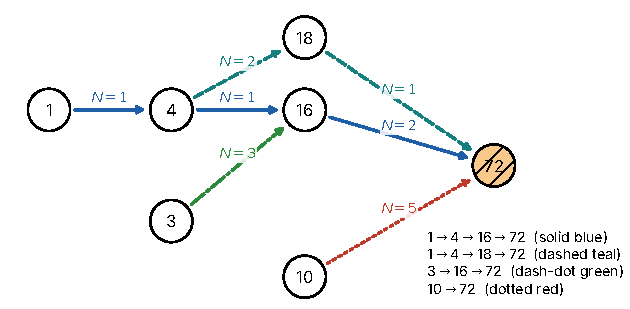
\includegraphics[width=0.92\textwidth]{fig02_four_histories_72}
\caption{\textbf{The four complete histories ending at $72$ (exact).} States are nodes, labels $N$ are edge labels. Source $1$: $1\to4\to16\to72$ (solid blue) and $1\to4\to18\to72$ (dashed teal); source $3$: $3\to16\to72$ (dash-dot green); source $10$: $10\to72$ (dotted red). Theorem illustrated: \cref{thm:predecessors}; \cref{ex:72}.}\label{fig:four}
\end{figure}
\begin{figure}[tbp]\centering
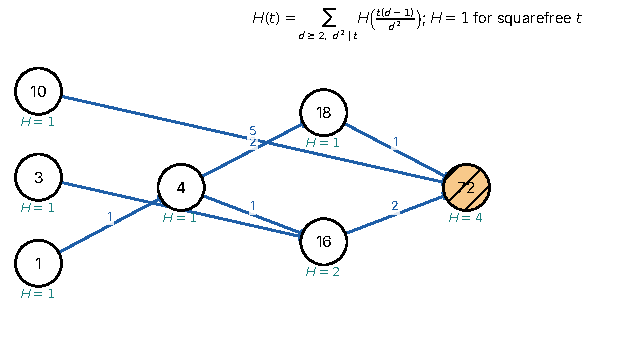
\includegraphics[width=\textwidth]{fig03_predecessor_graph}
\caption{\textbf{Predecessor graph of $72$ and the count recursion (exact).} Nodes are the ancestors of $72$; an edge $s\to t$ carries its label $N$; the number under a node is $H$ of that node, computed by the recursion of \cref{thm:predecessors}(c). $H(72)=4$.}\label{fig:predecessor}
\end{figure}

\subsection{Growth}
\begin{proposition}[lower bound for $72^r$]\label{prop:growth}
For every $r\ge1$, $H(72^r)\ge\binom{2r}{r}$.
\end{proposition}
\begin{proof}
Start from source $1$. Apply the label $1$ exactly $r$ times, reaching $4^r=2^{2r}$ (every state is divisible by the label $1$). We show that every arrangement of $r$ labels $1$ and $r$ labels $2$ is admissible from $4^r$. At a point where $a$ labels $1$ and $b$ labels $2$ have been applied so far, the $2$-adic valuation of the state is $2r+2a-b$, since a label $1$ adds $2$ and a label $2$ changes $v_2$ by $-1$ (the valuation of $R(2)=9/2$ is $-1$ at $2$). Before the $(b+1)$-st label $2$ we have $b\le r-1$, so $v_2\ge 2r-b\ge r+1\ge1$ and $2$ divides the state. The endpoint of any such arrangement is $4^r\cdot4^r\cdot(9/2)^r=72^r$ (the multiplier is $R(1)^rR(1)^rR(2)^r=4^{2r}(9/2)^r=(16\cdot9/2)^r=72^r$). Distinct arrangements are distinct words from one source, hence distinct histories; there are $\binom{2r}{r}$ of them, and the whole history $(1^r)\cdot(\text{arrangement})$ is from source $1$, which is squarefree, so these are complete.
\end{proof}
\prov{CW-0339}{D-T2}{PROVED}{FULL}

\begin{table}[tbp]\centering\small
\begin{tabular}{@{}lrrrrrr@{}}\toprule
$r$ & 1 & 2 & 3 & 4 & 5 & 6\\\midrule
$H(72^r)$ & 4 & 100 & 3\,601 & 194\,864 & 14\,177\,856 & 1\,258\,011\,667\\
$\binom{2r}{r}$ & 2 & 6 & 20 & 70 & 252 & 924\\\bottomrule
\end{tabular}
\caption{\textbf{Counts of complete histories ending at $72^r$ (finite-exact).} Values of $H$ from the recursion \cref{thm:predecessors}(c), computed exactly in this work and agreeing with the programme's records; the bound is \cref{prop:growth}. These are finite computations for $r\le6$: no growth law in $r$ is claimed (it is open, \cref{prob:growth}).}\label{tab:growth}
\end{table}
\begin{figure}[tbp]\centering
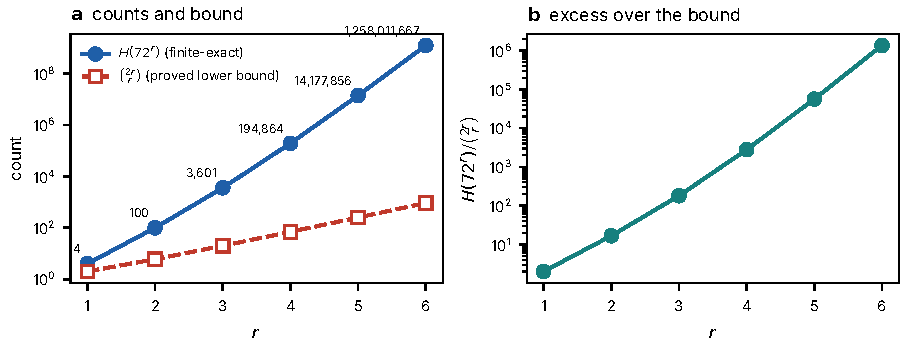
\includegraphics[width=0.95\textwidth]{fig04_growth}
\caption{\textbf{Growth of $H(72^r)$ and its lower bound (finite-exact values, proved bound).} (a) Counts for $r=1,\dots,6$ (circles, \cref{tab:growth}) against $\binom{2r}{r}$ (squares, \cref{prop:growth}). (b) The ratio; the bound is far from sharp.}\label{fig:growth}
\end{figure}
\noindent The figure above is \cref{fig:growth}; its caption states the exactness of what is drawn.
\begin{remark}
The values of \cref{tab:growth} for $r\le4$ were additionally confirmed by enumerating the histories explicitly; the values for $r=5,6$ rest on the recursion, which counts paths in an acyclic graph and whose correctness is \cref{thm:predecessors}.
\end{remark}
\begin{problem}[open: growth]\label{prob:growth}
Determine the asymptotics of $H(72^r)$ (and of the maximum cube dimension, \cref{sec:complexes}). Only the lower bound of \cref{prop:growth} and the finite values of \cref{tab:growth} are known here.
\end{problem}
\prov{CW-0514}{D-Q2}{OPEN}{OPEN}
